%!TEX root = ../../../super_main.tex
\subsection{Consistent Dialogs}
\label{sec:consistent_dialogs}

\todo{HOLMEHOLME Omskriv den her sektion således at brugen af dialog blvier beskrevet istedet for implementationen af dem. Det kan komme ned i implementations afsnittet.}

The pop-up dialogs have undergone a major overhaul during the second sprint. The previously implemented dialog (\androidinline{GDialog} see \figref{fig:gdialog}) was found to be inconsistent with the \giraf design manual. The overall idea was that all dialogs, across the \giraf-software suite, should be replaced with standard dialogs in order the give a consistent experience. 

\begin{figure}[!htbp]
    \centering
    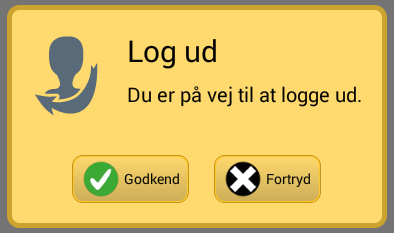
\includegraphics[width=0.4\textwidth]{sprint_two/giraf_components/gdialog}
    \caption{Old confirm dialog}
    \label{fig:gdialog}
\end{figure}


\subsubsection{Design}
We found that there were need of multiple common types of dialogs. The first being a simple notification dialog. which includes a title, a message, and a button for closing the dialog. The second is a confirmation dialog as seen in \figref{fig:giraf_confirm_dialog} provides an extra confirmation button and the possibility to provide an action for that button. In general it should be possible to add as many buttons to a dialog for other use cases. Besides this, it should be possible to have a dialog that can have more customizable content then just buttons and text. All of these dialogs should be able to close by clicking outside the dialog.

\begin{figure}[!htbp]
    \centering
    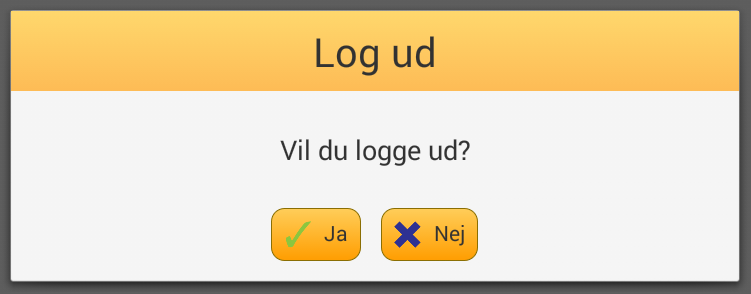
\includegraphics[width=0.7\textwidth]{sprint_two/giraf_components/giraf_confirm_dialog}
    \caption{Redesigned confirm dialog}
    \label{fig:giraf_confirm_dialog}
\end{figure}

\subsubsection{Implementation}

All dialogs should ideally look similar to provide a consistent experience. This was achieved by letting all dialogs inherit from the same abstract class called \androidinline{GirafDialog} which implements functionality and visuals used in all the subclasses. There were created some specialized classes of the dialog, for the various use cases. The general approach for callback from these classes is the implemented should use some interface to ensure that action in the dialog can handled somewhere.

\todo{HOLMEHOLME end.}